% !TeX root = ../paper.tex

\section{Evaluation and Discussion}
\label{sec:results}

Results are organized by hypothesis. All figures report the per-task paired change
between the no-feedback baseline and the final iteration, across the three loop
configurations of \cref{sec:configs}. Two significance tests are used: the
Wilcoxon signed-rank test~\citep{wilcoxon1945signedrank} for the paired metric
changes (H1, H2), and an exact (binomial) variant of the McNemar
test~\citep{mcnemar1947} for the change in
functional correctness (H3). Both are non-parametric
and paired, which suits the bounded, non-normal metrics and the small sample.
Because a family of twelve tests is reported---the three primary metrics and the
correctness test, each across the three configurations---every $p$-value is
additionally assessed against a Bonferroni-corrected
threshold~\citep{dunn1961multiple} of
$\alpha^\ast = 0.05/12 = 0.00417$ to control the family-wise error rate. A
summary is given in \cref{tab:results}, where the $p$-values that remain
significant after this correction are marked with a dagger ($\dagger$).

Every value below measures the archived runs (\cref{sec:artifacts}) and recomputes
from the retained solutions exactly; a fresh run reproduces the direction and
approximate size of these effects but not their precise figures, so the discussion
rests on the sign, significance, and ordering of the effects rather than their exact
magnitudes.

\subsection{Baseline Results}
The baseline model solves \textbf{28 of 63 tasks} (44\,\%) under the MBPP+ oracle.
Its generated code already scores well: the median baseline Maintainability Index
is 95.4, and 46 of 63 solutions reach at least 90, though \cref{sec:results}
shows how much of that is comment credit.

\begin{table*}[t]
  \centering
  \caption{Effect of three feedback-loop configurations on 63 tasks. Metric
    columns report the median per-task change (final $-$ baseline) and the
    two-sided Wilcoxon $p$; correctness reports the baseline$\rightarrow$final
    pass count and the exact McNemar-type $p$. For MI, higher is better (a negative
    change is a decline); for CC and CogC, lower is better (a negative change is
    an improvement). A dagger ($\dagger$) marks $p$-values below the
    Bonferroni-corrected threshold $\alpha^\ast = 0.05/12 = 0.00417$.}
  \label{tab:results}
  \begin{tabular}{lccccc}
    \toprule
    & \textbf{Correctness} & \multicolumn{2}{c}{\textbf{MI (H1)}}
      & \textbf{CC (H2)} & \textbf{CogC (H2)} \\
    \cmidrule(lr){3-4}
    \textbf{Configuration} & base$\rightarrow$final ($p$) & med.\ $\Delta$ & $p$
      & med.\ $\Delta$ ($p$) & med.\ $\Delta$ ($p$) \\
    \midrule
    Unguarded, comment-stripping    & $28\!\to\!23$ ($.13$)  & $-3.0$ & $<.001^\dagger$ & $0$ ($.0036^\dagger$) & $-1$ ($<.001^\dagger$) \\
    Unguarded, comment-preserving   & $28\!\to\!22$ ($.07$)  & $-3.4$  & $<.001^\dagger$ & $0$ ($.02$)    & $0$ ($<.001^\dagger$) \\
    Correctness-guarded             & $28\!\to\!\mathbf{29}$ ($1.0$) & $-1.1$ & $<.001^\dagger$ & $0$ ($.03$)  & $0$ ($<.001^\dagger$) \\
    \bottomrule
  \end{tabular}
\end{table*}

\subsection{Effect on Maintainability (H1)}
The Maintainability Index does not improve under any configuration; it declines
significantly in all three (\cref{fig:deltas}, left). The
decline is, tellingly, essentially the same whether the refactor prompt
strips comments or preserves them: a median of $-3.0$ points in the
comment-stripping configuration versus $-3.4$ in the comment-preserving one. A
direct per-task comparison of the two confirms this; their final Maintainability
Indices do not differ significantly (Wilcoxon $p=.13$). That similarity is not,
however, evidence that comments are irrelevant. Comment density is high at the
baseline (mean 49\,\%) and moves sharply both ways, to 19\,\% under the stripping
prompt and to 85\,\% under the preserving one, while the Index's comment term is
non-monotonic and peaks near 58\,\%~\citep{coleman1994maintainability,radon_docs}.
A baseline sitting at that maximum therefore loses points in \emph{either}
direction: the term falls by a mean of 14.2 points under stripping and 8.8 under
preserving, and at the median baseline ratio it contributes about 29 points on its
own, so the ceiling is largely its artifact too. Comment handling is thus the dominant driver of every MI figure
reported here; with the term held fixed, the mean structural component instead rises
slightly in all three configurations. Combined with the validity limitations
documented by Heitlager et al.~\citep{heitlager2007maintainability}, the decline is
best read as evidence that the MI is an unsuitable outcome metric here, not that
the loop harms maintainability. The Index is therefore reported for completeness
but treated as secondary; cognitive complexity is the primary maintainability
signal in what follows.

\subsection{Effect on Complexity (H2)}
Cognitive complexity improves. Although its median change is zero or $-1$---most of
the 63 tasks are simple enough that little or no reduction is possible---the change
is highly significant in every configuration ($p<.001$; \cref{fig:deltas}, right),
because among the tasks that do change, reductions dominate overwhelmingly. In the
correctness-guarded configuration, 26 tasks reduce their cognitive complexity and
only one increases it. Of the 63 tasks, 36 show no change at all; the Wilcoxon
test discards these zero-difference pairs as uninformative and evaluates only the
27 tasks that did change. Among those 27, a 26:1 split in favor of reductions is
highly unlikely to arise by chance, which is what drives the significance despite
the zero median. The effect is strongest where there is structural headroom:
in the higher-complexity stratum of the guarded loop the median change is $-1$ and
remains significant ($p=.002$), though this stratum analysis is exploratory and is
not part of the corrected family. Individual cases are substantial; for example one task falls from a
cognitive complexity of 15 to 2 while remaining correct. \Cref{fig:cogcscatter}
shows this task-by-task: most points lie on or below the diagonal, and the largest
reductions occur at the highest baseline values.

Cyclomatic complexity behaves similarly but more weakly. Its reductions are
smaller: at the uncorrected level they are significant in all three configurations
(comment-stripping $p=.0036$, comment-preserving $p=.02$, guarded $p=.03$), but
after Bonferroni correction only the comment-stripping configuration remains
significant. This divergence between the two complexity
metrics is expected: the feedback
prompt targets nested and redundant control flow, which cognitive complexity
penalizes more directly than cyclomatic complexity.

\begin{figure*}[t]
  \centering
  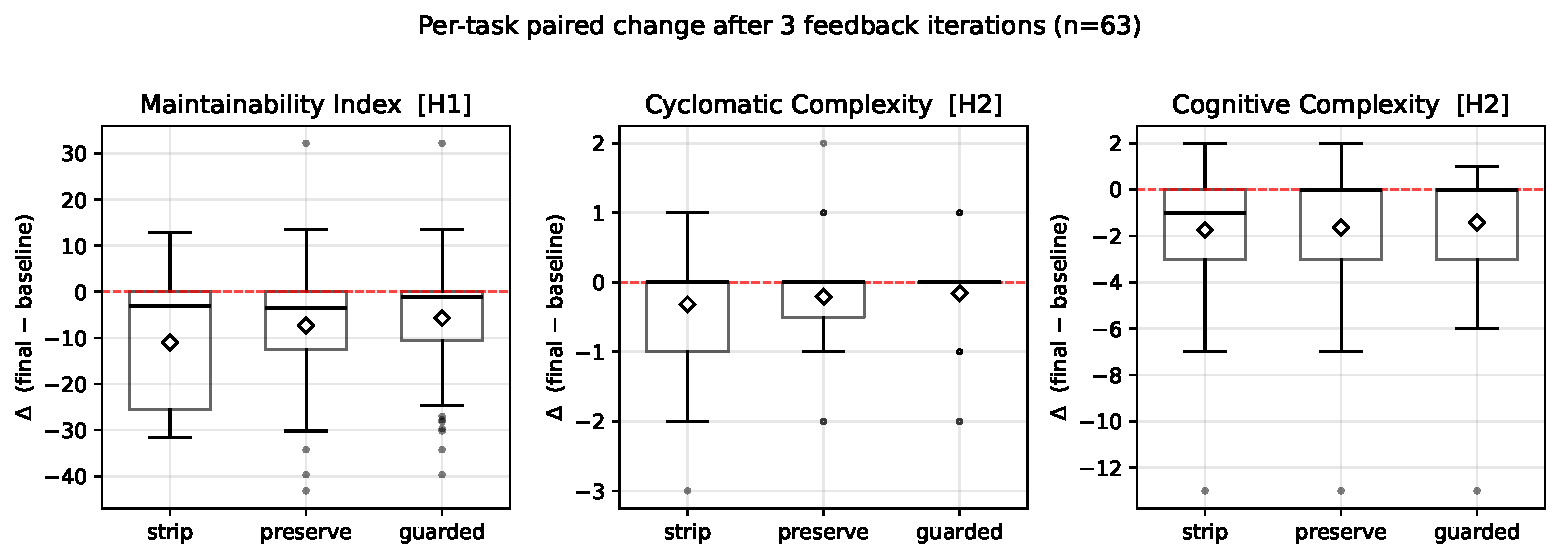
\includegraphics[width=\textwidth]{figures/fig_delta_boxplots}
  \caption{Per-task paired change (final $-$ baseline) for each metric and
    configuration. The dashed line marks no change; diamonds mark means. The
    Maintainability Index (left) declines modestly and by a similar amount in
    every configuration; cyclomatic complexity (middle) barely moves; cognitive
    complexity (right) concentrates below zero, indicating reductions.}
  \label{fig:deltas}
\end{figure*}

\subsection{Qualitative Example: De-nesting Reduces Cognitive Complexity}
\label{sec:example}
\Cref{fig:example} makes the aggregate cognitive-complexity result concrete on a
single task (Mbpp/245, the maximum sum of a bitonic subsequence). The baseline
solution (a) computes two auxiliary arrays with doubly nested loops whose inner
bodies guard an accumulator update with a compound \texttt{if}; this deep nesting
is what cognitive complexity penalizes, and the solution scores 15. Under the
correctness-guarded loop the model replaced each inner loop with a generator
expression inside \texttt{max(\dots, default=\dots)}, removing the nesting while
computing the same values; cognitive complexity falls to 2 and the solution still
passes the MBPP+ oracle. This single example also illustrates why the two
complexity metrics diverge (\cref{sec:supp}): \emph{cyclomatic} complexity is unchanged at 10; the number of
independent branches is essentially the same, yet \emph{cognitive} complexity drops by 13, because it is the nesting, not the branch
count, that the refactor removed. The Maintainability Index rises from 78.5 to
92.0 and the code shortens from 18 to 9 lines, but the readability gain that
cognitive complexity captures is the substantive change.

\begin{figure*}[t]
  \centering
  \begin{minipage}{\textwidth}
  \footnotesize (a) Baseline solution --- cognitive complexity 15, cyclomatic 10, MI 78.5.
  \begin{lstlisting}[basicstyle=\ttfamily\footnotesize,numbers=none]
def max_sum(arr):
    n = len(arr)
    inc = [0] * n
    dec = [0] * n
    for i in range(n):
        inc[i] = arr[i]
        for j in range(i):
            if arr[i] > arr[j] and inc[i] < inc[j] + arr[i]:
                inc[i] = inc[j] + arr[i]
    for i in range(n-1, -1, -1):
        dec[i] = arr[i]
        for j in range(i+1, n):
            if arr[i] > arr[j] and dec[i] < dec[j] + arr[i]:
                dec[i] = dec[j] + arr[i]
    max_sum_bitonic = 0
    for i in range(n):
        max_sum_bitonic = max(max_sum_bitonic, inc[i] + dec[i] - arr[i])
    return max_sum_bitonic
  \end{lstlisting}
  \vspace{0.4em}
  \footnotesize (b) After correctness-guarded feedback --- cognitive complexity 2, cyclomatic 10, MI 92.0.
  % scriptsize, not footnotesize: the two generator-expression lines are ~97 chars
  % and wrapped mid-subscript at footnotesize, which read as broken Python. The code
  % is the model's output and is shown verbatim, so it is the type size that gives.
  \begin{lstlisting}[basicstyle=\ttfamily\scriptsize,numbers=none]
def max_sum(arr):
    n = len(arr)
    inc = [arr[i] for i in range(n)]
    dec = [arr[i] for i in range(n)]
    for i in range(1, n):
        inc[i] = max((inc[j] + arr[i] for j in range(i) if arr[i] > arr[j]), default=arr[i])
    for i in range(n-2, -1, -1):
        dec[i] = max((dec[j] + arr[i] for j in range(i+1, n) if arr[i] > arr[j]), default=arr[i])
    return max(inc[i] + dec[i] - arr[i] for i in range(n))
  \end{lstlisting}
  \end{minipage}
  \caption{A representative correctness-preserving refactor from the guarded loop
    (comments omitted for space). Replacing the nested inner loops with generator
    expressions removes the deep nesting: cognitive complexity falls from 15 to 2
    while cyclomatic complexity is unchanged at 10, and all MBPP+ tests still pass.}
  \label{fig:example}
\end{figure*}

\subsection{Effect on Functional Correctness (H3)}
The unguarded configurations trend toward losing correct solutions, from 28 down
to 23 and 22, but neither change is statistically significant (McNemar
$p=.13$ and $p=.07$). This is an important limit on the claim: at this sample size,
the data do not establish that the unguarded loop significantly harms correctness,
only that it does not improve it and shows a downward trend. The counts are
nonetheless worth reading in proportion rather than in the aggregate: of the 28
solutions that were correct at the baseline, 6 and 7 respectively were broken by refactoring, between a fifth and a quarter of everything the model had already got
right. Whether or not that reaches significance on 63 tasks, it is the practical
risk the gate is designed to remove. The
correctness-guarded configuration ends at 29 correct solutions with zero
regressions. This is a design guarantee rather than a
statistical result: the gate rejected 13 of 189 refactors that broke behavior---12
of them in the lower-complexity stratum, where the model tends to over-refactor
simple functions---and rolled each one back to its last correct version.

The gate also works in the other direction, which is why the guarded run ends
\emph{above} its baseline. On one task (Mbpp/167, ``next power of 2'') the baseline
solution initialized its accumulator to $0$ and then doubled it with a left shift,
so the loop condition never advanced and the oracle recorded a timeout as a
failure. A later refactor initialized the accumulator to $1$ instead, which is
correct; the gate verified the fix against the oracle and locked it in. The gate is
therefore a ratchet on correctness rather than merely a brake: it can hold or
improve the pass count but, by construction, never reduce it.

\begin{figure}[t]
  \centering
  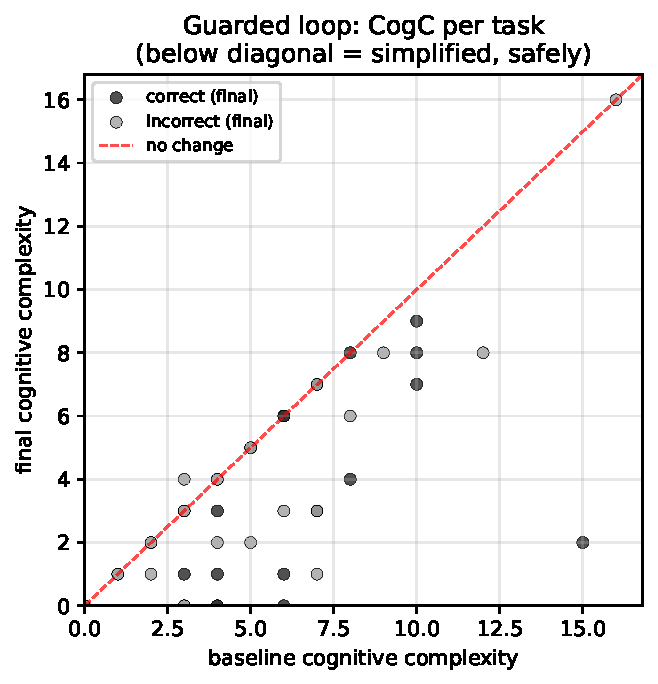
\includegraphics[width=0.72\columnwidth]{figures/fig_cogc_scatter}
  \caption{Guarded loop: baseline versus final cognitive complexity for all 63
    tasks. Points below the diagonal are simplified. No task that passes the
    baseline oracle fails at the final iteration; tasks failing both are included.}
  \label{fig:cogcscatter}
\end{figure}

\subsection{Iteration Dynamics}
\label{sec:trajectory}
\Cref{fig:trajectory} tracks how the metrics evolve across the three feedback
iterations. The effect is concentrated almost entirely in the first iteration:
mean cognitive complexity and the Maintainability Index both move at iteration~1
and then change little through iterations~2 and~3, in every configuration. This
holds at the task level too---among the tasks whose cognitive complexity changes at
all, most reach their final value already after one iteration (27 of 39 for
comment-stripping, 24 of 32 for comment-preserving, and 20 of 27 for the guarded
loop), with only a handful first improving at the second or third iteration. The
loop therefore behaves close to a single-shot refactor. The three-iteration budget
is consequently not a binding constraint for most tasks; it mainly provides
headroom for the minority that improve later and, in the guarded loop, for retries
after a rejected refactor. A smaller cap would capture most of the observed
benefit, and a substantially larger one would be unlikely to add much, which is the empirical justification for the fixed cap of three.

\begin{figure}[t]
  \centering
  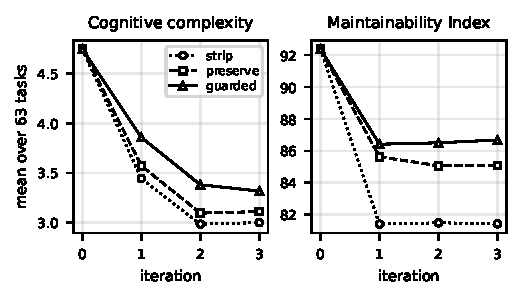
\includegraphics[width=\columnwidth]{figures/fig_trajectory}
  \caption{Mean cognitive complexity (left) and Maintainability Index (right) at
    each iteration (0~=~baseline), one line per configuration. Both change chiefly
    at the first iteration and then plateau, in all three configurations.}
  \label{fig:trajectory}
\end{figure}

\subsection{Supplementary Metrics}
\label{sec:supp}
Beyond the three primary metrics, the pipeline records lines of code (LOC),
Halstead volume and effort, and Pylint issue counts at no additional measurement
cost. These are reported here as descriptive corroboration; they are not part of
the hypothesis family and carry no significance test. Because all three
configurations share the identical baseline generation, their baseline medians
coincide (\cref{tab:supp}).

Two of these measures independently reinforce the interpretation of the primary
results. First, source lines of code barely move and do so uniformly; the median falls from 9 to 7 in every configuration, including comment-stripping. Because SLOC excludes comments and multiline strings, that uniformity says nothing
about comment volume; the component analysis above shows the comment ratio is what
drives the MI decline. Second, Halstead
volume and effort are effectively flat (median change $\approx 0$) in every
configuration: the loop restructures control flow without materially changing
program size or vocabulary. This is exactly the signature expected when cognitive
complexity, which penalizes nesting and control structure, falls while size-based
measures do not, and it argues against the complexity reduction being an artifact
of the code simply getting smaller. Pylint issue counts decline modestly (median 6
to 4--5). This last figure carries the least evidential weight of any reported
here, because Pylint is the loop's own feedback source: the model is told which
findings it triggered, so a subsequent fall in those counts partly restates the
instruction rather than measuring an independent improvement. It is noted as a
side effect and nothing in the argument depends on it.

\begin{table}[t]
  \centering
  \footnotesize
  \setlength{\tabcolsep}{4pt}
  \caption{Supplementary metrics (descriptive; not in the hypothesis family),
    reported as median baseline$\rightarrow$median final per configuration
    (comment-stripping / comment-preserving / correctness-guarded). Baselines
    coincide because the three configurations share one baseline generation. LOC
    is source lines of code (\texttt{radon raw} SLOC); Pylint issues is the total
    of convention, refactor, warning, and error messages.}
  \label{tab:supp}
  \begin{tabular}{lccc}
    \toprule
    & \textbf{Strip} & \textbf{Preserve} & \textbf{Guarded} \\
    \midrule
    LOC (SLOC)      & $9\!\to\!7$         & $9\!\to\!7$         & $9\!\to\!7$ \\
    Halstead vol.   & $62.3\!\to\!57.1$   & $62.3\!\to\!64.7$   & $62.3\!\to\!64.7$ \\
    Halstead eff.   & $140.1\!\to\!142.4$ & $140.1\!\to\!142.4$ & $140.1\!\to\!142.4$ \\
    Pylint issues   & $6\!\to\!4$         & $6\!\to\!4$         & $6\!\to\!5$ \\
    \bottomrule
  \end{tabular}
\end{table}

\subsection{Synthesis}
Taken together, the three configurations answer the research question with a
qualified yes. The feedback loop produces a statistically significant reduction in
cognitive complexity, one that survives Bonferroni correction for multiple
comparisons in every configuration, without a statistically significant loss of
functional correctness, and the correctness-guarded variant turns the absence of
regression into a guarantee. It does not improve the Maintainability Index, but that decline tracks the Index's
comment term rather than structural quality, which, with its documented validity
limitations~\citep{heitlager2007maintainability}, makes it a sign of the metric's
unsuitability here rather than a failing of the method. The practical cost of the guarantee is small: the
guarded loop forgoes a few complexity reductions that were only achievable by
altering behavior (12 tasks reduced cyclomatic complexity, against 16 under the
comment-preserving unguarded loop that shares its prompt), in exchange for
eliminating every correctness regression. A follow-up
ablation (\cref{sec:blind}) shows that this complexity reduction does not even
require showing the model its own code.

\subsection{Feedback Content: Is the Generated Code Needed?}
\label{sec:blind}
The configurations above all feed the model its previous code together with the
static-analysis findings. To test whether the code is what drives the effect, a
\emph{code-blind} variant withholds the previous code and supplies only the
scalar findings of the previous attempt, asking for a fresh, simpler solution
(\cref{sec:configs}). Because this variant addresses a distinct, secondary
research question rather than the pre-specified primary hypotheses, its tests are
treated as a separate multiplicity family with their own correction. It is
compared against the
code-aware comment-preserving loop, though the two prompts also differ in comment
handling, so this ablates the feedback package rather than code visibility alone.

The central result is that the code is \emph{not} needed for the complexity
reduction. The code-blind loop reduces cognitive complexity significantly (median
$-1$, $p<.001$), and a per-task comparison of the two final versions shows no
significant difference from the code-aware loop ($p=.65$); the Maintainability
Index declines almost identically in both ($-3.4$ points). Withholding the code
does, however, make the unguarded loop noisier on correctness: because it
re-derives each solution from scratch rather than editing a known-correct one, it
regresses eight tasks and repairs three, against the code-aware loop's seven and
one (\cref{tab:blind}). The code-blind loop ends at 23 correct solutions and the code-aware at 22, neither change is statistically
significant, but the code-blind
loop clearly takes larger correctness risks in both directions.

This is precisely the risk the correctness gate is designed to absorb, and it
does. The guarded code-blind loop rejects every behavior-breaking regeneration, so
it records \emph{zero} regressions; and because blind regeneration is a coarser
operation that occasionally rewrites a broken baseline into a correct solution, it
even repairs three tasks, ending at 31 correct, slightly above the guarded
code-aware loop's 29. Its cognitive-complexity reduction is preserved ($p=.005$)
and again statistically indistinguishable from the code-aware loop ($p=.43$). The
practical conclusion is that showing the model its own code is unnecessary for the
complexity benefit, and that a lightweight correctness gate makes code-blind
regeneration not merely safe but, on this sample, marginally better for
correctness.

\begin{table}[t]
  \centering
  \footnotesize
  \setlength{\tabcolsep}{2pt}
  \caption{Code-blind ablation (secondary family, $n=63$), compared with the
    code-aware comment-preserving loop. Correctness reports
    baseline$\rightarrow$final with the exact McNemar-type $p$; CogC and MI report the
    median per-task change and the Wilcoxon $p$. A dagger ($\dagger$) marks
    $p$-values below this family's Bonferroni threshold
    $\alpha^\ast = 0.05/8 = 0.00625$.}
  \label{tab:blind}
  \begin{tabular}{lccc}
    \toprule
    \textbf{Configuration} & \textbf{Correct.} & \textbf{CogC} & \textbf{MI} \\
    & base$\rightarrow$final & med.\ $\Delta$ ($p$) & med.\ $\Delta$ ($p$) \\
    \midrule
    Code-aware, ungu.  & $28\!\to\!22$ & $0$ ($<.001^\dagger$) & $-3.4$ ($<.001^\dagger$) \\
    Code-blind, ungu.  & $28\!\to\!23$ & $-1$ ($<.001^\dagger$) & $-3.4$ ($.002^\dagger$) \\
    Code-aware, guard. & $28\!\to\!29$ & $0$ ($<.001^\dagger$) & $-1.1$ ($<.001^\dagger$) \\
    Code-blind, guard. & $28\!\to\!\mathbf{31}$ & $0$ ($.005^\dagger$) & $-1.4$ ($.008$) \\
    \bottomrule
  \end{tabular}
\end{table}
